\chapter{Fundamentos teóricos y estado del arte} \label{chp:state-of-the-art}

En este capítulo se cubre el estado del arte de la energía solar \gls{fotovoltaica} y, particularmente, de la \gls{librería} \pvlibpy{}. Se podrá encontrar en las siguientes secciones:

\begin{itemize}

      \item \fullref{sct:energia-solar}: explica el estado actual de la energía solar \gls{fotovoltaica} y su fundamento teórico base.

      \item \fullref{sct:simulaciones}: detalla las herramientas de \gls{simulación} utilizadas en el sector fotovoltaico y el marco general de comparación de la librería \pvlibpy{}.

      \item \fullref{sct:pvlib}: presenta las características de la biblioteca \pvlibpy{}.

\end{itemize}

%%%%%%%%%%%%%%%%%%%%%%%%%%%%%%%%%%%%%%%%%%%%%%%%%%%%%%%%%%%%%%%%%%%%%%%%%%%%%%%%
%%%%%%%%%%%%%%%%%%%%%%%%%%%%%%%%%%%%%%%%%%%%%%%%%%%%%%%%%%%%%%%%%%%%%%%%%%%%%%%%

\section{La energía solar fotovoltaica} \label{sct:energia-solar}

En esta sección se presentará el estado del arte de las diferentes tecnologías, estudios y sistemas relacionados con la energía solar fotovoltaica.

La energía solar \gls{fotovoltaica} es una tecnología que convierte la \gls{radiación solar} en electricidad utilizando células solares mediante el \gls{efecto fotoeléctrico} \cite[][pp. 701-706]{böer2002survey}.
Este fenómeno consiste en la generación de una corriente eléctrica cuando la luz incide sobre un material \gls{semiconductor} y excita los electrones de la \gls{banda de valencia} a la \gls{banda de conducción}. Esta excitación genera un \gls{par electrón-hueco} que se separa por la acción de un campo eléctrico externo (en cuyo caso no se produce energía neta positiva) o mediante la distribución de cargas en un \gls{semiconductor} p-n, que permite la extracción de energía. Este último caso es el de aplicación en células solares fotovoltaicas, pues la intención es obtener energía eléctrica.

Existen varias tecnologías de células solares, como las de silicio, las de película delgada y, las más experimentales, de concentración y de otros materiales orgánicos y multiunión, que se agrupan en generaciones \cite{Shubbak_2019}. Cada generación responde a una serie de características e implantación en el mercado, donde destacan:

\begin{itemize}
      \item Primera generación: células de \gls{silicio monocristalino} y \gls{silicio policristalino}.
            Se encuentran bien implantadas en el mercado y son las más utilizadas en aplicaciones fotovoltaicas. Según el límite teórico que calcularon Shockley y Queisser en 1961, el silicio es el material más apropiado para la fabricación de células solares, ya que su \gls{banda prohibida} de $1.1 eV$ es la que mejor se ajusta al máximo de la \gls{radiación solar} \cite[][p. 1126]{böer2002survey}. Sin embargo, presentan un coste de producción moderado y un alto uso de material. El límite de eficiencia teórico obtenido por los anteriores autores es del 33.7\% \cite{Shockley_Queisser_1961} para \gls{colectores} planos y células solares de una sola unión, es decir, que no tratan ni con \gls{sistemas de concentración} ni \gls{células multiunión o tándem}.
      \item Segunda generación: células de película delgada, como las de telururo de cadmio ($CdTe$), las de di-seleniuro de cobre, indio y galio (\textit{Copper indium gallium selenide}, $CuInGaSe_2$), las de arseniuro de galio (\textit{Gallium arsenide}) ($GaAs$) y las de \gls{silicio amorfo} ($\text{a-Si:H}$).
            Destacan por ser de capa delgada (\textit{thin-film}) y, consecuentemente, más baratas de producir por el bajo uso de material, si bien pueden llegar a ser composiciones de materiales más caros.
            Nótese que el \gls{silicio amorfo} es ampliamente utilizado, en especial en aplicaciones de baja potencia, como calculadoras, pero su eficiencia es inferior a las células de silicio cristalino.
      \item Tercera generación: células de concentración, células de múltiples uniones y \gls{células orgánicas}.
            Se encuentran en fase de investigación y desarrollo, y se caracterizan por su alta eficiencia y coste elevado.
            Por un lado destacan la tecnología de concentración, que emplea lentes para concentrar la luz solar en células de alta eficiencia, normalmente de múltiples uniones, que pueden alcanzar eficiencias superiores al 40\% \cite[][Tabla 5]{Green_Dunlop_Yoshita_Kopidakis_Bothe_Siefer_Hao_2024}. Se emplean sistemas ópticos para disminuir el uso de material \gls{semiconductor}, que el principal factor de coste en estas células.
\end{itemize}

Cada una tiene sus propias características y aplicaciones específicas. Las células de primera y segunda generación son las más comunes en aplicaciones fotovoltaicas, mientras que las de tercera generación se encuentran en fase de investigación y desarrollo. El lector puede remitirse a \cite{Shubbak_2019} para una revisión más detallada de cada grupo y las peculiaridades de cada material.

En la siguiente sección se hace una revisión de algunos conceptos y efectos que intervienen en la producción de energía fotovoltaica.

\subsection{Conceptos y efectos en los sistemas fotovoltaicos}

Una gran cantidad de factores influyen en la utilidad y el retorno energético y económico de un sistema de generación fotovoltaico. Entender estos factores es fundamental para el diseño y la operación de sistemas PV. En las siguientes líneas se presentan algunos que son de especial interés.

\subsubsection{Radiación y espectro solar}

La radiación es una onda electromagnética que se propaga a la velocidad de la luz y transmite energía. Como la misma luz visible, que cuenta con colores, la radiación que proviene del Sol también tiene diferentes longitudes de onda. Cuenta con regiones como la luz visible, el \gls{ultravioleta} y el \gls{infrarrojo}. La cantidad de energía que hay por cada ``color'' o \gls{longitud de onda} se conoce como espectro solar.

Por un lado, la \gls{irradiancia} (radiación incidente) tiene unidades de potencia por unidad de área $[W/m^2]$, y el espectro solar es la distribución de este mismo por cada \gls{longitud de onda}, por lo que se mide en $[W/m^2/nm]$.

Dependiendo de las condiciones atmosféricas, la cantidad de masa de aire que debe atravesar y la presencia de unos gases u otros en diferentes concentraciones, la \gls{radiación extraterrestre} sufre una reducción en ciertas longitudes de onda. Se debe, entre otros fenómenos, al scattering o la reflexión que producen algunos gases de la atmósfera. La forma que toma la \gls{radiación solar} en la superficie terrestre es lo que se conoce como espectro solar terrestre. El \gls{estándar} ASTM G173-03 \cite{astm_g173-03} describe un \gls{espectro estándar} para analizar la radiación solar en la superficie terrestre. En la siguiente figura se puede observar el espectro solar terrestre global, el directo que proviene del Sol sin contar con reflexiones, y el extraterrestre:

\begin{figure}[H]
      \centering
      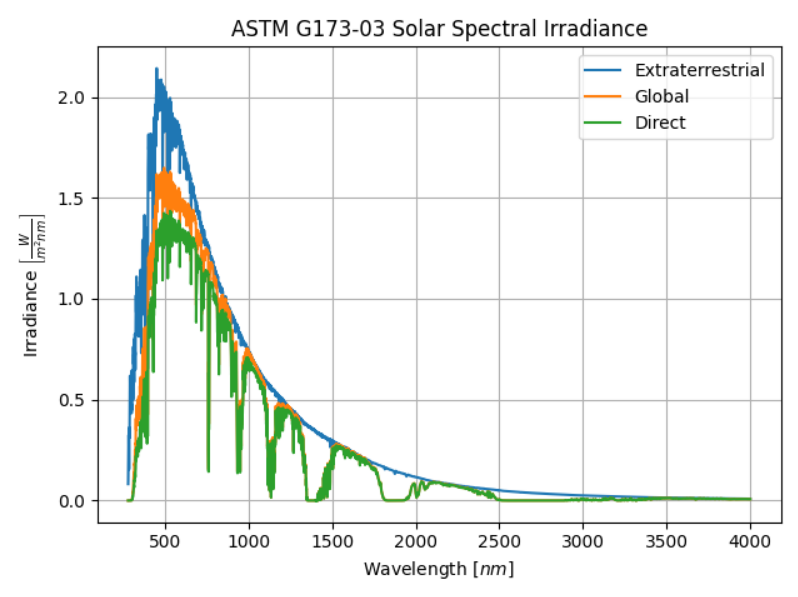
\includegraphics[width=0.7\textwidth]{./images/SoA_irrad/astm_g173-03.png}
      \caption{Espectro solar terrestre. Fuente: ejemplo de este documento en \ref{sct:doc_ej_espectro_astm} añadido a \pvlibpy{}.}
      \label{fig:solar_spectrum}
\end{figure}

Para muchos análisis de radiación, se emplea más la potencia incidente por unidad de área $[W/m^2]$ que el espectro, en $[W/m^2/nm]$, pues la forma del espectro no tiene grandes variaciones y el volumen de datos de este último es varios órdenes de magnitud mayor.

\subsubsection{Medida de la radiación solar}

Hay tres medidas de la radiación solar que son interesantes para normalizar la forma en que se mide y posteriormente deducir la que pueda llegarle a un colector fotovoltaico. Estas son:

\begin{itemize}
      \item Global en una superficie horizontal (\textit{\gls{GHI}}, \textit{Global Horizontal Irradiance}): es la radiación que llega a una superficie horizontal.
      \item Directa normal (\textit{\gls{DNI}}, \textit{Direct Normal Irradiance}): es la radiación proveniente del disco solar que llega a una superficie perpendicular a los rayos solares.
      \item Difusa en una superficie horizontal (\textit{\gls{DHI}}, \textit{Diffuse Horizontal Irradiance}): es la radiación que llega a una superficie horizontal tras ser dispersada por la atmósfera.
\end{itemize}

A partir de estas medidas, se puede modelar cuál será la radiación solar en una superficie inclinada y orientada en función de los ángulos de inclinación y \gls{acimut} de los módulos, mediante modelos científicos conocidos como de \gls{transposición}. Estas tres componentes se relacionan mediante:

\begin{equation} \label{eq:ghi_dni_dhi}
      GHI = DNI \cdot \cos(\theta) + DHI
\end{equation}

Donde $\theta$ es el ángulo cenital del Sol (o sea, el ángulo entre la línea vertical y su posición), que normalmente se obtiene con modelos de posición solar a partir del instante de tiempo y la localización geográfica.

La ecuación \ref{eq:ghi_dni_dhi} es interesante porque facilita comprobar la calidad de las medidas si existen las tres, y si solo existen dos de ellas, permite deducir la tercera.

Las unidades de las componentes de la irradiancia solar son $\si{\watt\per\meter\squared}$.

Los instrumentos de medida en campo que permiten obtener estos parámetros son \gls{piranómetros} para medir \textit{\gls{GHI}}; \gls{pirheliómetros}, para \textit{\gls{DNI}}; y \gls{piranómetros} con bola de sombra del disco solar para \textit{\gls{DHI}}. En la figura \ref{fig:irrad_componentes} se puede observar la relación entre las componentes de la radiación solar y los instrumentos de medida:

\begin{figure}[H]
      \centering
      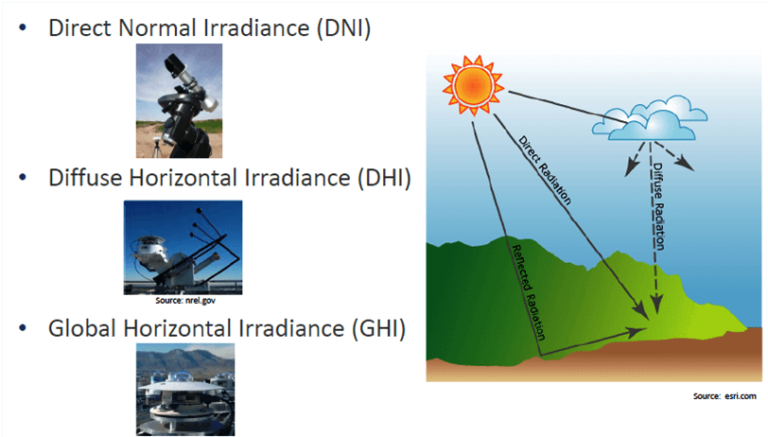
\includegraphics[width=0.7\textwidth]{./images/SoA_irrad/dni-dhi-ghi-1-768x437.png}
      \caption{Componentes de la radiación solar y los instrumentos de medida. Fuente: Yellow Haze Sustainable, 2017. \href{http://web.archive.org/web/20230624215046/https://yellowhaze.in/wp-content/uploads/2017/01/dni-dhi-ghi-1-768x437.png}{Enlace}.}
      \label{fig:irrad_componentes}
\end{figure}

\subsubsection{Transposición e irradiancia en un colector plano}

Al orientar un colector fotovoltaico, la radiación que llega a este dependerá de la inclinación y el \gls{acimut} del colector. La radiación que llega a un colector plano se puede descomponer en tres componentes: la radiación \gls{directa}, la radiación \gls{difusa} -del cielo- y la radiación \gls{reflejada} -del suelo-:

\begin{itemize}
      \item Componente \gls{directa} o circunsolar: es la radiación que llega directamente del Sol sin reflexiones. Es la mayoritaria en días despejados.
      \item Componente difusa: es la radiación que llega de la atmósfera tras ser dispersada por las partículas en suspensión y las nubes.
      \item Componente difusa del suelo y superficies circundantes, o albedo: es la reflejada por el entorno, como el suelo, la naturaleza u otras estructuras de la instalación fotovoltaica, como hileras de módulos adicionales. Se puede asumir que es nula para un \gls{módulo} \gls{monofacial} orientado horizontalmente hacia arriba.
\end{itemize}

Para calcular estas componentes en el plano del generador a partir de las medidas de radiación solar vistas en la sección anterior, se emplean modelos de \gls{transposición}. Se tratan de relaciones geométricas entre la \gls{irradiancia} en el plano horizontal y el inclinado. El \gls{modelo} más común es el de Pérez \cite{Perez_Ineichen_Seals_Michalsky_Stewart_1990}, pero hay otros como el Pérez-Driesse que solventa un problema de continuidad \cite{Driesse_Jensen_Perez_2024}.

\subsubsection{Células fotovoltaicas}

Anteriormente se detallaba sobre los materiales y algunas tecnologías de la fotovoltaica. Esta sección se centra en células planas convencionales, en especial las de silicio, que son las más extendidas.

Estos dispositivos semiconductores son similares en construcción a un \gls{diodo}, donde la unión toma una gran superficie que es la que se usa para recolectar la radiación. Se considera que la radiación que llega es proporcional a la corriente que se genera: esta se denomina fotocorriente. Sin embargo, por tratarse de un \gls{diodo}, este deja pasar corriente en el sentido inverso al de la generación de energía, lo que implica que hay pérdidas debidas a la propia construcción del \gls{diodo}. El siguiente circuito eléctrico representa un \gls{modelo} simplificado de una célula solar:

\begin{figure}[H]
      \centering
      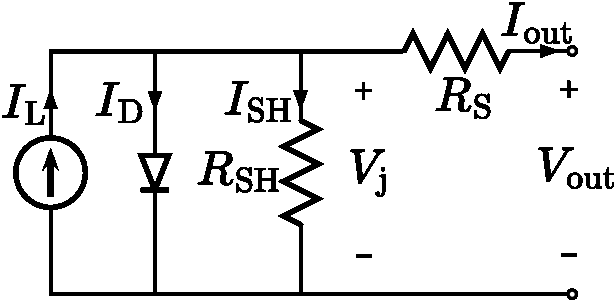
\includegraphics[width=0.5\textwidth]{./images/SoA_irrad/Solar_cell_equivalent_circuit_latex.png}
      \caption{\Gls{modelo} simplificado de un \gls{diodo} de una \gls{célula solar}. Fuente: Em3rgent0rdr, ``Solar cell equivalent circuit latex'', 2024. \href{https://commons.wikimedia.org/w/index.php?curid=149538519}{Enlace}.}
      \label{fig:solar_cell_model}
\end{figure}

$I_L$ representa la fotocorriente, $I_D$ la corriente que circula por el \gls{diodo}, $I_{SH}$ la corriente de pérdidas en paralelo por la resistencia ``\gls{shunt}'' $R_{SH}$, e $I_{OUT}$ la corriente de salida que circula por $R_{S}$, la resistencia en serie. Estas resistencias de pérdidas se deben a la construcción de las células solares, las uniones entre el \gls{semiconductor} y los contactos metálicos, y a la propia resistencia del material \gls{semiconductor}.

\subsubsection{Curva I-V: la característica de una célula solar}

Del circuito anterior se deduce por tanto que a igualdad de \gls{irradiancia} incidente, y por ende, de fotocorriente, la tensión y la corriente que se extraerá dependerá del punto de trabajo de la célula. Cuanta más corriente se extraiga, más caerá la tensión antes del \gls{diodo} y este hará que se pierda menos corriente en la propia célula, pero también que se reduzca esta tensión.

La curva que se observa al cambiar la tensión de trabajo de la célula y medir la corriente que sale de ella se conoce como \gls{curva I-V}. En la figura \ref{fig:iv_curve} se puede observar una curva I-V típica de una célula solar:

\begin{figure}[H]
      \centering
      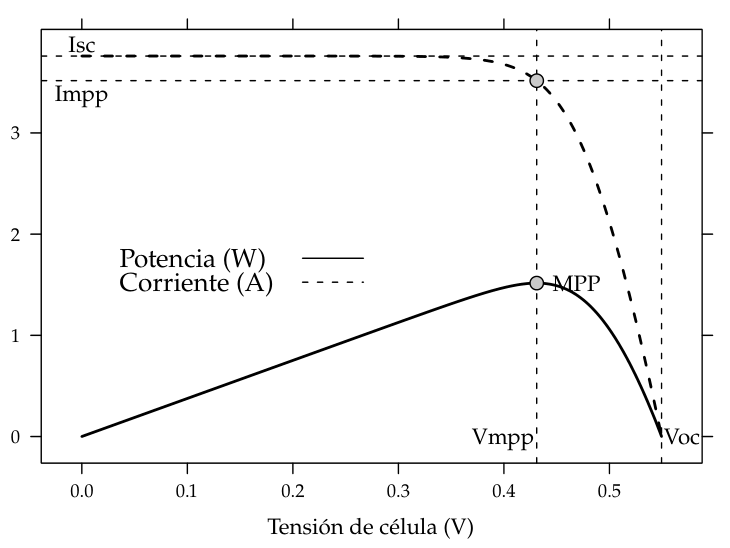
\includegraphics[width=0.7\textwidth]{./images/SoA_irrad/Solar_Cell_I-V_Curve_Schematic.png}
      \caption{\Gls{curva I-V} de una \gls{célula solar}. Fuente: Óscar Perpiñán, ``Energía Solar Fotovoltaica'', 2020. \cite[Fig. 4.6]{Perpinan2020}.}
      \label{fig:iv_curve}
\end{figure}

La curva sólida inferior es el producto de la tensión y la corriente en cada punto, la potencia de salida. Esta curva se conoce como \gls{curva P-V}. Se puede observar que la máxima potencia de salida está en un punto que se conoce como punto de máxima potencia (MPP, \textit{Maximum Power Point}). Este punto es el que interesa para la producción de energía eléctrica.

Una tensión de célula que no excede 0.7 V es típica de las hechas con silicio. Esta tensión es muy pequeña para ser extraída eficientemente, por ello que se deben crear módulos fotovoltaicos con muchas de ellas para solventar este problema.

\subsubsection{Respuesta espectral y eficiencia cuántica externa}

En realidad la \gls{radiación solar} no es homogénea en todas las longitudes de onda, y una \gls{célula solar} tampoco es igual de sensible a ellas. La curva de \gls{respuesta espectral} se define como la capacidad de convertir una potencia lumínica a determinada \gls{longitud de onda} en una corriente. Esta métrica se cuantifica en $[A/W]$ y depende del material y otros aspectos constructivos, según se puede observar en la figura \ref{fig:spectral_response}:

\begin{figure}[H]
      \centering
      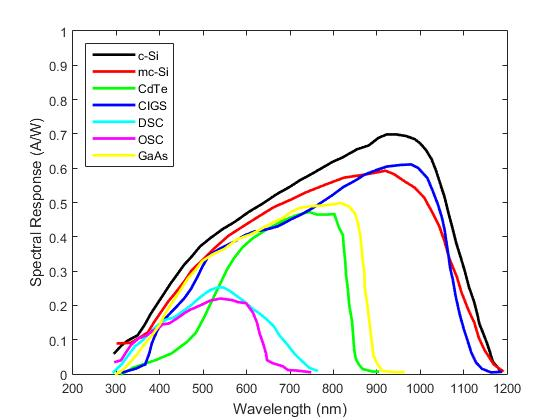
\includegraphics[width=0.7\textwidth]{./images/SoA_irrad/Spectral_Response_PV.jpg}
      \caption{\Gls{respuesta espectral} de una \gls{célula solar}. Fuente: Sandia National Laboratories, ``Image of Spectral\_Response\_PV'', 2024. \href{https://pvpmc.sandia.gov/modeling-guide/2-dc-module-iv/effective-irradiance/spectral-response/}{Enlace}.}
      \label{fig:spectral_response}
\end{figure}

La \gls{eficiencia cuántica externa} $EQE(\lambda)$ es una medida similar, pero en este caso se mide cuál es la fracción de fotones incidentes a una \gls{longitud de onda} determinada que se convierten en electrones de fotocorriente. Es un número adimensional y se relaciona con la \gls{respuesta espectral} $SR(\lambda)$ mediante la ecuación:

\begin{equation} \label{eq:relacion_sr_eqe}
      SR(\lambda) = \frac{q \cdot \lambda}{h \cdot c} \cdot EQE(\lambda)
\end{equation}

Donde $q$ es la carga electrostática del electrón, $h$ es la constante de Planck, $c$ es la velocidad de la luz y $\lambda$ la \gls{longitud de onda} para cada punto de las curvas.

\subsubsection{Módulos}

Las células solares se conectan en serie para que la tensión de todas las células se sume y se pueda extraer una tensión mayor \cite{victoria2024fundamentals}, con una corriente que es la misma que la de una sola célula. Al no aumentar la corriente, se evitan pérdidas mayores debidas al \gls{efecto Joule} por la resistencia de las conexiones.

Un \gls{módulo} también presenta una curva I-V, que idealmente será la misma que la de una célula pero escalada en la tensión en función del número de células. En realidad, por pequeñas variaciones en la construcción de las células y la conexión de estas, la \gls{curva I-V} de un módulo no es exactamente la misma que la de una célula. Además, este problema se ve muy agravado cuando la \gls{irradiancia} no es homogénea en todas las células del módulo y puede suponer un riesgo en el caso extremo de haber sombras. Por esta razón se emplean diodos de derivación o \textit{bypass} para evitar que una célula sombreada disipe energía en forma de calor y se dañe ella o el propio módulo.

Un ejemplo de curvas I-V y P-V de un grupo de módulos -de dos \glspl{string} en paralelo, de 4 módulos cada una- en condiciones de ausencia de sombra y con sombras parciales se puede observar en la figura \ref{fig:iv_pv_curve}:

\begin{figure}[H]
      \centering
      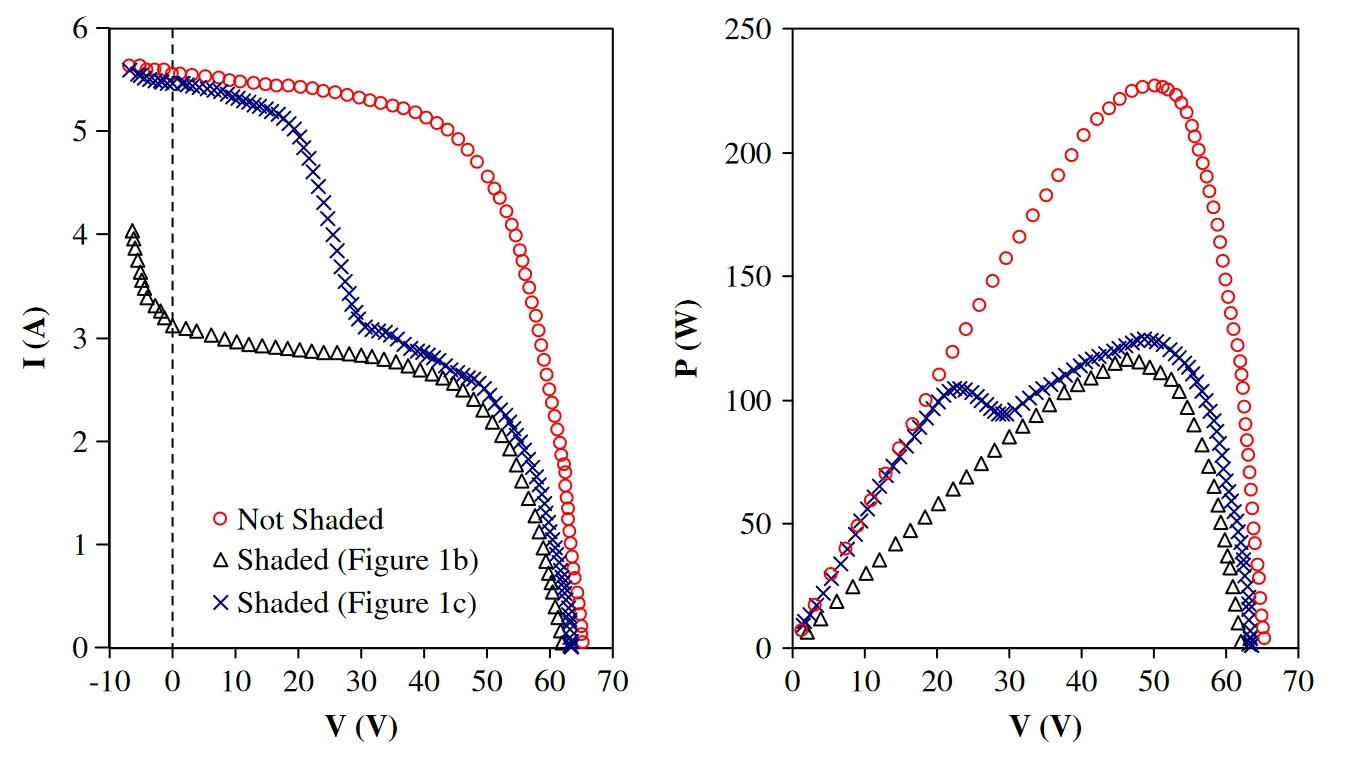
\includegraphics[width=0.7\textwidth]{./images/SoA_irrad/IV_PV_Curve_Module_Under_Shading.jpg}
      \caption{Curvas I-V y P-V de un grupo de módulos en distintas condiciones de sombra. Fuente: F. Martínez-Moreno et al., ``Experimental model to estimate shading losses on PV arrays'', 2010. \cite[Fig. 3]{Martínez-Moreno_Muñoz_Lorenzo_2010}.}
      \label{fig:iv_pv_curve}
      Sin sombra (rojo/$\bigcirc$), 3 módulos de una misma \gls{string} sombreados (negro/$\triangle$) y dos módulos de una misma \gls{string} parcialmente sombreados (azul/$\times$).
\end{figure}

Es por esto que el efecto que produce una sombra parcial sobre un módulo o un conjunto de módulos es muy perjudicial. Se ahonda en este tema en más detalle en la sección \ref{sssct:efecto-sombra}.

\subsubsection{Efecto de la temperatura}

La temperatura hace que el \gls{diodo} en el equivalente circuital en \ref{fig:solar_cell_model} conduzca mucho más, aumentando las pérdidas que se disiparían en este. Por ello, la eficiencia de las células disminuye con la temperatura \cite{Perpinan2020}. La temperatura de las células se estima mediante modelos empíricos basados en la disipación de calor por conducción, convección y radiación.

Por esta razón se plantean sistemas fotovoltaicos algo más inusuales, como los \gls{sistemas flotantes} sobre cuerpos de agua, que permiten refrigerar las células con el agua.

\subsubsection{Sombra y diodos de \textit{bypass}} \label{sssct:efecto-sombra}

Es necesario tener en cuenta factores de pérdidas como la \gls{sombra}, la suciedad o la nieve en el diseño de sistemas fotovoltaicos. Cualquier obstrucción de la radiación sobre una célula genera una afección a la producción parcial o completa de un \gls{módulo}. Las células se conectan en serie, por lo que la corriente que pasa por una es la misma que pasa por todas. Si una célula está sombreada, las demás células forzarán la corriente que pasa por ella, haciendo que esta se comporte como una \gls{carga} y disipe energía en forma de calor \cite{Perpinan2020}.

Esta energía disipada en la célula sombreada se convierte en calor, y puede llegar a dañar el módulo.

Este efecto se conoce como \textit{hot spot} y puede dañar la integridad del módulo. Se emplean diodos de derivación o \textit{bypass} para mitigarlo. Estos permiten que la corriente mayoritaria de las células más iluminadas circule por el \gls{diodo} y no se vea limitada por las células sombreadas. En las aplicaciones industriales típicas, sistemas de autoconsumo en la superficie terrestre, se emplea un \gls{diodo} para proteger a un grupo de células. Normalmente se encuentran tres por módulo; se trata del compromiso entre el coste de poner diodos adicionales, la mitigación de los \textit{hot spots} y las pérdidas por sombreado.

\subsubsection{Sistemas fotovoltaicos}

Se llama \gls{sistema fotovoltaico} al acople de los módulos junto con componentes y dispositivos eléctricos para hacer que la energía producida por los paneles sea utilizable. Entre este equipamiento adicional destacan:

\begin{itemize}
      \item Inversores: son los encargados de convertir la corriente continua producida por los módulos en corriente alterna, que es la que se emplea en la red eléctrica.
      \item Convertidores DC-DC: permiten adaptar la tensión y la corriente de los módulos a la que se necesita en el sistema.
      \item Seguidor del punto de máxima potencia: el MPP varía en función de las condiciones de \gls{irradiancia} y temperatura de los módulos, por lo que se emplean sistemas que maximizan la producción de energía mediante algoritmos que hayan este punto. Normalmente bien el convertidor DC-DC o el inversor incorpora esta función.
      \item Seguidores solares: son estructuras que orientan los módulos hacia el Sol a lo largo del día para maximizar la producción de energía.
      \item Sistemas de almacenamiento: permiten almacenar la energía producida por los módulos para su uso posterior mediante baterías.
      \item Sistemas de monitorización: para controlar el rendimiento de los módulos y detectar fallos en el sistema.
\end{itemize}

No todos los sistemas incorporan los equipos mencionados anteriormente. Se han desarrollado diferentes configuraciones, cada una con sus propias ventajas y dificultades, como sistemas conectados a la red, \gls{sistemas autónomos} y \gls{sistemas de bombeo} \cite{Perpinan2020}:

\begin{itemize}
      \item Sistemas conectados a la red: son los más comunes y se emplean para inyectar energía en la red eléctrica. Se necesitan \gls{inversores} que conviertan la corriente continua en alterna.
      \item Sistemas autónomos: se emplean en lugares remotos donde no llega la red eléctrica o es inestable el acceso. Usan \gls{sistemas de almacenamiento} y de gestión de la energía.
      \item Sistemas de bombeo: se emplean para bombear agua durante las horas diurnas a un depósito. Solo requieren un seguidor del punto de máxima potencia que trabaje adecuadamente con el motor de la bomba.
\end{itemize}

En todos estos casos, es recomendable contar con herramientas de simulación y análisis para evaluar el rendimiento de los sistemas, optimizar su diseño y diagnosticar problemas a partir de datos meteorológicos, entre otros.

\section{Simulación de sistemas fotovoltaicos} \label{sct:simulaciones}

La \gls{simulación} de sistemas es fundamental para diseñarlos y dimensionarlos adecuadamente.

Toda simulación de un \gls{sistema fotovoltaico} habitual necesita calcular la radiación solar incidente en la superficie de los módulos. Las variables de partida de una simulación siempre involucran valores meteorológicos como la radiación solar, la temperatura ambiente y la velocidad del viento \cite{Perpinan2020}. Adicionalmente, se emplean modelos empíricos para obtener valores como la radiación solar extraterrestre en la superficie de la atmósfera y deducir otros parámetros de entrada para el resto del flujo de cálculos, en función de los instantes de tiempo que se vayan a analizar.

La infografía \ref{fig:pv_simulation_flow} detalla los efectos que normalmente se tienen en cuenta para simular todo un sistema fotovoltaico:

\begin{figure}[H]
      \centering
      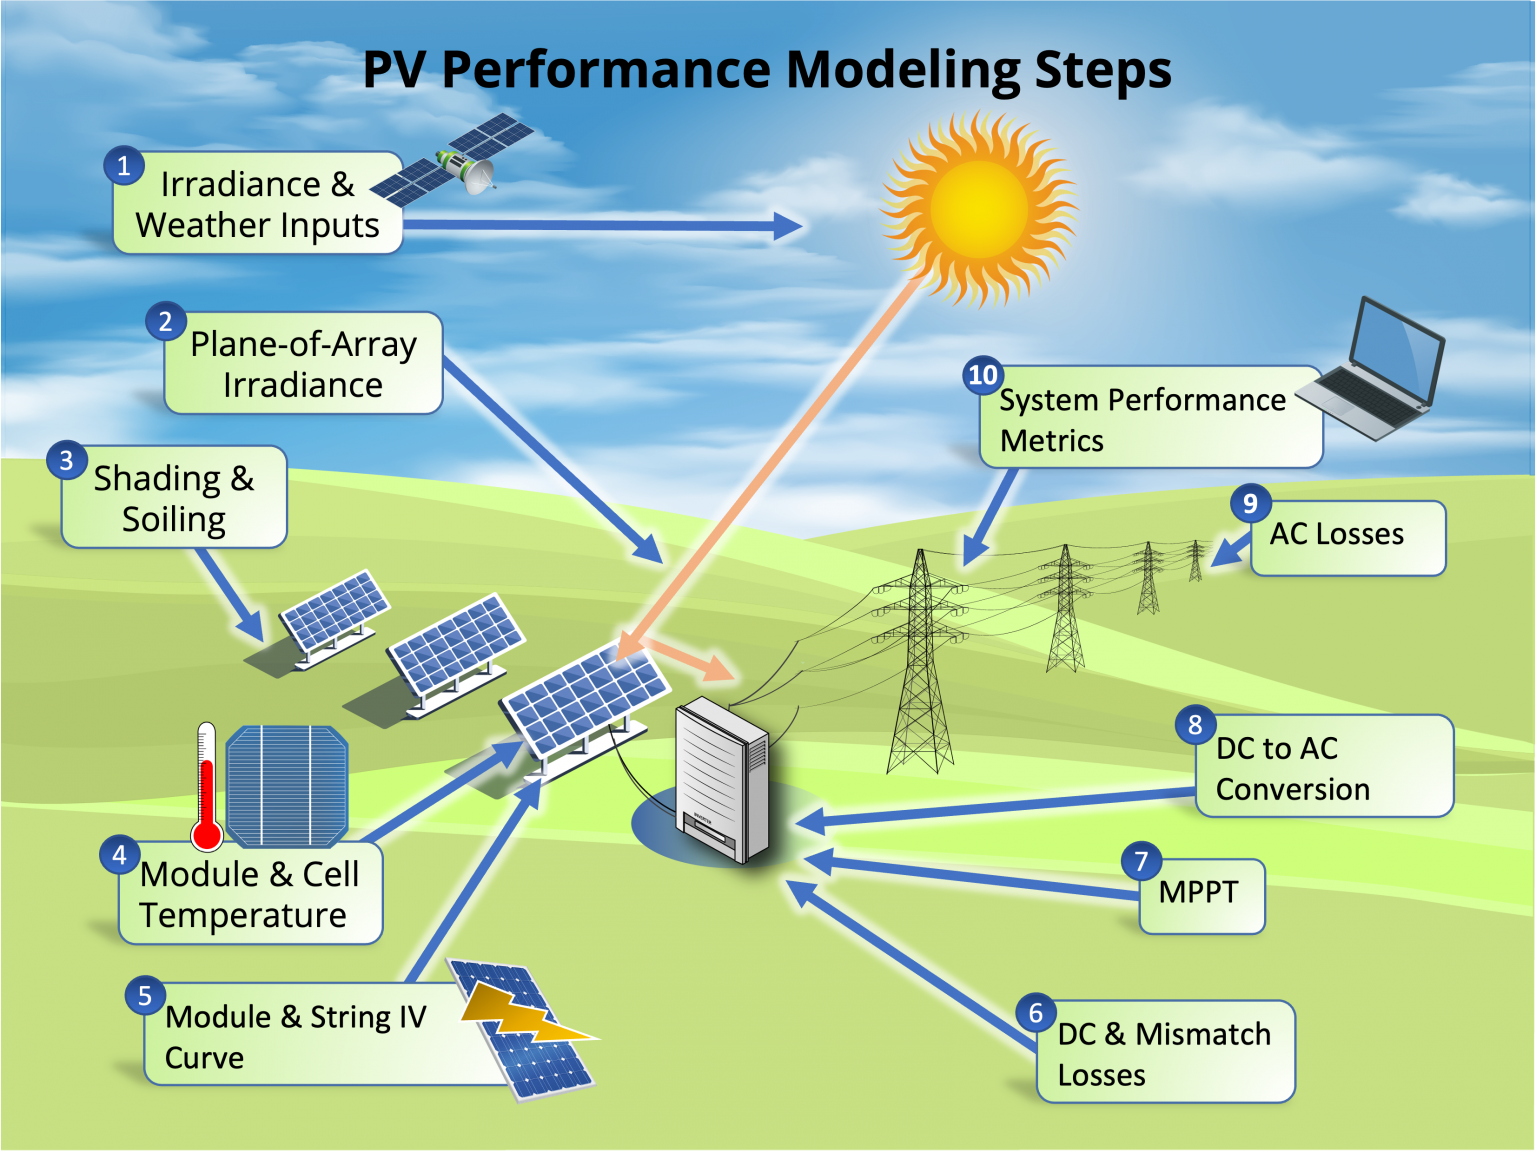
\includegraphics[width=0.7\textwidth]{./images/SoA_irrad/pv_simulation_flow.png}
      \caption{Flujo de cálculo en la simulación de un sistema fotovoltaico. Fuente: Sandia National Laboratories, PV Performance Modeling Collaborative (PVPMC), 2024. \href{https://pvpmc.sandia.gov/}{Enlace}.}
      \label{fig:pv_simulation_flow}
\end{figure}

El primer punto son datos meteorológicos y las componentes de la irradiancia.

Se comprueba la necesidad de establecer numéricamente las coordenadas del Sol en el cielo para hacer cálculos y comprobar las medidas. Se emplea un sistema de \gls{coordenadas esféricas} con dos ángulos: el \gls{cenit} y el \gls{acimut}. El cenit es el ángulo entre una línea vertical y el Sol, y el acimut es el ángulo entre el norte y la proyección del Sol en el plano horizontal. Debe denotarse que en ocasiones se emplea el \gls{ángulo de elevación}, que es el ángulo entre el Sol y el plano horizontal; es decir, el ángulo complementario al cenit. En la figura \ref{fig:solar_angles} se pueden observar los ángulos solares mencionados, donde $\beta_s$ es la elevación y $\gamma_s$ es el acimut:

\begin{figure}[h]
      \centering
      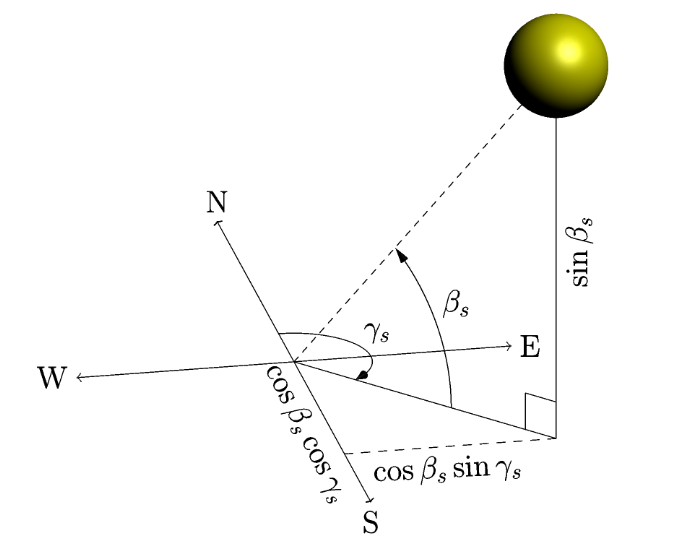
\includegraphics[width=0.6\textwidth]{./images/SoA_irrad/Anderson_Mikofski_Fig2.png}
      \caption{Ángulos solares. Fuente: K. Anderson, M. Mikofski, ``Slope-Aware Backtracking for Single-Axis Trackers'', 2020. \cite[Fig. 2]{Anderson_Mikofski_2020}.}
      \label{fig:solar_angles}
\end{figure}

Por definición de \gls{ángulos complementarios}, el \gls{cenit} $\theta_s$ se relaciona con la elevación $\beta_s$ mediante la ecuación $\theta_s = 90^\circ - \beta_s$.

A partir de los valores de irradiancia solar \textit{\gls{GHI}}, \textit{\gls{DNI}} y \textit{\gls{DHI}}, se puede calcular la irradiancia por componentes que llega a la superficie de los módulos: la \gls{directa}, la \gls{difusa} y la \gls{reflejada}. La componente directa es la que proviene de la dirección del sol y llega directamente a la superficie de los módulos, la irradiancia difusa es la que proviene del resto del cielo y se dispersa en todas direcciones, y la irradiancia reflejada o \gls{albedo} es la que proviene de la reflexión y emisión de radiación sobre superficies cercanas. Estas componentes se suman para obtener la radiación total incidente en la superficie de los módulos, que es la que se emplea para calcular la producción de energía.

El siguiente paso es cuantificar el efecto de la temperatura: la eficiencia de las células disminuye conforme aumenta la temperatura debido a la \gls{recombinación interna} y la reducción de la \gls{banda prohibida}. La temperatura de las células se estima mediante modelos empíricos que, como mínimo, dependen de la estructura de montaje de los \glspl{módulo}, la irradiancia, la temperatura ambiente y la velocidad del viento.

Algunos factores de pérdidas se toman en cuenta en este instante como el \gls{ajuste espectral}, corrección por no-uniformidad de la radiación, la suciedad y la nieve, que suelen afectar a la irradiancia incidente. Por otra parte, otros factores de pérdidas somo la \gls{sombra} y las pérdidas en los conductores por \gls{efecto Joule}, se aplican respecto la potencia de salida de los módulos.

En general, dependerá del modelo en cuestión y cómo se haya planteado originalmente, pero cabe destacar esta diferencia entre aplicar modelos a la radiación incidente o a la potencia de salida.

A continuación, se modela la integración de los \gls{inversores}, \gls{sistemas de almacenamiento} o \gls{transformadores}, si procede en cada caso.

Finalmente se obtiene la producción horaria de energía, que se puede integrar en el tiempo para obtener la producción, asignarle un retorno económico y estimar la viabilidad del proyecto de instalación fotovoltaica \cite{Rosa-Clot_Tina_2020}.

\subsection{Herramientas de simulación}

La importancia de simulaciones y análisis previo a la implantación de sistemas fotovoltaicos tanto para promotores, operaciones de financiación y diseñadores ha dado lugar a múltiples herramientas \gls{software} y modelos como PVWatts, PVGIS, PV-Online, PV*SOL, PVsyst, System Advisor Model (SAM) y muchas más \cite{stein_models_2009, Kumar_2017}. Normalmente estas herramientas propietarias ponen el foco en calcular el rédito energético y económico de una instalación fotovoltaica, pero no en el desarrollo de la investigación y validación de modelos científicos.

La Sección \ref{sct:pvlib} mostrará que la librería \pvlibpy{}, y su predecesor en \gls{MATLAB}, se centra en la investigación y validación de modelos científicos para la simulación de sistemas fotovoltaicos, mientras que se obvia el cálculo de coste y rédito económico.
